\chapter{Copulas and Its Applications}

Copulas (or couplae in Latin) are an interesting mathematical tool to represent correlations between probability distributions. They can be used to describe complex dependencies in multivariate risk models, when more basic tools such as multivariate Gaussian distributions are inappropriate. Another commonly used application is sampling from correlated random variables.

In this Chapter the copula concept is reviewed and some example applications are shown. 
Before going into the copulas we need to learn how to transform a distribution into another using the \emph{probability integral transform}. 

\section{Distribution Transformation}\label{distribution-transformation}

Distribution transformation is a very useful tool which will be
extensively used with the copula concept that we discuss in the next
Section. The technique we are going to outline transforms every random
variable, regardless its distribution, into uniform and vice versa and is called
\emph{probability integral transform} or (percentile-to-percentile
transform).

Computationally, this method involves computing the quantile function (see Section~\ref{quantile-function}) of
a distribution, in other words, computing the cumulative
distribution function ($F(x)$) of a distribution (which maps a number
to a probability between 0 and 1) and then inverting that
function. We won't go into the details but we will just show few
examples of how this can be done in \(\tt{python}\).

Imagine we want to transform an uniform distribution into a Gaussian.
The transformation takes uniform samples of a number \(u\) between 0 and
1, interpreted as a probability, and then returns $F^{-1}(u)$. 

Table~\ref{tab:transformation} shows samples taken from the
uniform distribution and their representation on the standard normal
distribution determined using the algorithm explained above.

\begin{table}[h]
  \centering
  \begin{tabular}{|c|c|}
    \hline
    \(\mathbf{u}\) & \(\mathbf{F^{-1}(u)}\) \\
    \hline
    0.5 & 0 \\
    \hline
    .975 & 1.95996 \\
    \hline
    .995 & 2.5758 \\
    \hline
    .999999 & 4.75342 \\
    \hline
    \(1-2^{-52}\) & 8.12589 \\
    \hline
  \end{tabular}
  \caption{Comparison of values of the uniform distribution and the corresponding Gaussian quantiles.}
\label{tab:transformation}
\end{table}

Now let's see how this can be done with \texttt{python}. The first step is to sample
uniformly distributed values between 0 and 1. This can be done either using \texttt{random.random} like in Section~\ref{pseudo-random-numbers} or with \texttt{scipy.stats.uniform}. Each distribution defined in \texttt{scipy.stats} has a convenient method \texttt{rvs(size=aSize)} (random variable sample) to sample from it as many time as specified by the arguments \texttt{size}. Usually the second method is preferred since it exploits \texttt{numpy.array} and let us avoid a lot of for-loop cycles.

In any case in the left plot of Fig.~\ref{fig:uniform_and_gauss} the resulting distribution is shown.

\begin{tcolorbox}[breakable, size=fbox, boxrule=1pt, pad at break*=1mm,colback=cellbackground, colframe=cellborder]
\begin{Verbatim}[commandchars=\\\{\}]
\PY{k+kn}{from} \PY{n+nn}{scipy} \PY{k}{import} \PY{n}{stats}
\PY{n}{x} \PY{o}{=} \PY{n}{stats}\PY{o}{.}\PY{n}{uniform}\PY{p}{(}\PY{l+m+mi}{0}\PY{p}{,} \PY{l+m+mi}{1}\PY{p}{)}\PY{o}{.}\PY{n}{rvs}\PY{p}{(}\PY{l+m+mi}{10000}\PY{p}{)}
\end{Verbatim}
\end{tcolorbox}

Next we want to transform these samples so that instead of uniform they
are normally distributed. As we have seen, see Section~\ref{quantile-function} the transform that does this
is the inverse of the cumulative density function of the normal 
distribution, or \((\tt{ppf(x))}\) in \texttt{oython}. 

In the right plot of Fig.~\ref{fig:uniform_and_gauss} the Gaussian obtained 
with the code below is shown

\begin{figure}[h]
  \centering
  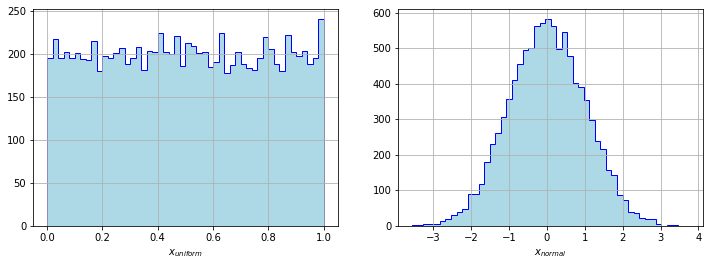
\includegraphics[width=1.\textwidth]{figures/uniform_gauss.png}
  \caption{On the left the generated uniform distribution, on the right its Gaussian transform.}
  \label{fig:uniform_and_gauss}
\end{figure}

\begin{tcolorbox}[breakable, size=fbox, boxrule=1pt, pad at break*=1mm,colback=cellbackground, colframe=cellborder]
\begin{Verbatim}[commandchars=\\\{\}]
\PY{n}{norm} \PY{o}{=} \PY{n}{stats}\PY{o}{.}\PY{n}{norm}\PY{p}{(}\PY{p}{)} 
\PY{n}{x\PYZus{}trans} \PY{o}{=} \PY{n}{norm}\PY{o}{.}\PY{n}{ppf}\PY{p}{(}\PY{n}{x}\PY{p}{)}
\end{Verbatim}
\end{tcolorbox}

If we plot them together in a 2D plot we can get a sense of what is
going on using the inverse CDF transformation.
Indeed it stretches the outer regions of the uniform to yield a
normal distribution. The transformation is shown in Fig.~\ref{fig:uniform_to_gauss}. 
    
\begin{figure}[htbp]
  \centering
  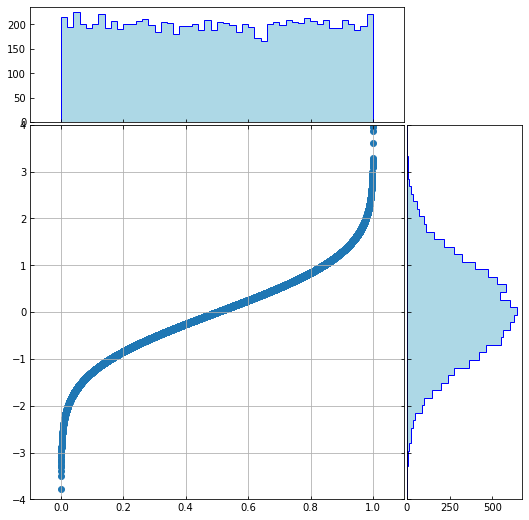
\includegraphics[width=0.5\textwidth]{figures/lesson6_7_0.png}
  \caption{2D plot showing the transformation that maps our initial uniform distribution to the resulting Gaussian.}
  \label{fig:uniform_to_gauss}
\end{figure}
    
The nice thing of this technique is that it can be used
for any arbitrary (uni-variate) probability distribution, like for
example \href{https://en.wikipedia.org/wiki/Student\%27s\_t-distribution}{t-Student}
or \href{https://en.wikipedia.org/wiki/Gumbel_distribution}{Gumbel}.
A similar transformation from uniform to t-Student is shown in Fig.~\ref{fig:uniform_to_tstudent}.

\begin{tcolorbox}[breakable, size=fbox, boxrule=1pt, pad at break*=1mm,colback=cellbackground, colframe=cellborder]
\begin{Verbatim}[commandchars=\\\{\}]
\PY{n}{t} \PY{o}{=} \PY{n}{stats}\PY{o}{.}\PY{n}{t}\PY{p}{(4}\PY{p}{)} 
\PY{n}{x\PYZus{}trans} \PY{o}{=} \PY{n}{t}\PY{o}{.}\PY{n}{ppf}\PY{p}{(}\PY{n}{x}\PY{p}{)}
\end{Verbatim}
\end{tcolorbox}

\begin{figure}[htbp]
  \centering
  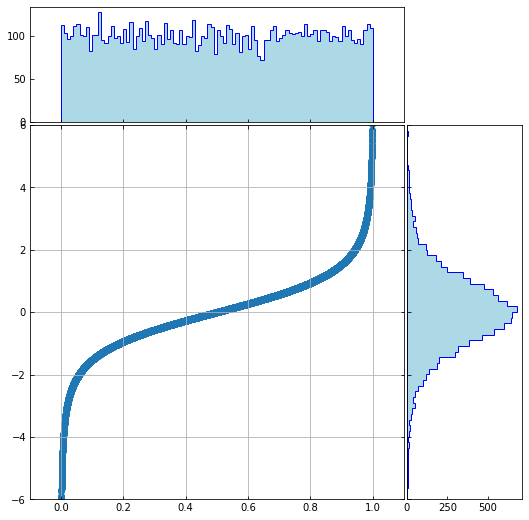
\includegraphics[width=0.5\textwidth]{figures/lesson6_9_0.png}
  \caption{2D plot showing the transformation that maps a uniform distribution to a t-Student.}
  \label{fig:uniform_to_tstudent}
\end{figure}

Clearly to do the opposite transformation, from an arbitrary distribution
to the uniform, we can just apply the inverse of the inverse CDF, that is the CDF itself\ldots
In such a way we can go from distribution A to distribution B passing through 
a uniform distribution rather quickly. An example is shown in Figure~\ref{fig:a_to_b_to_a}.

\begin{figure}[htbp]
	\centering
	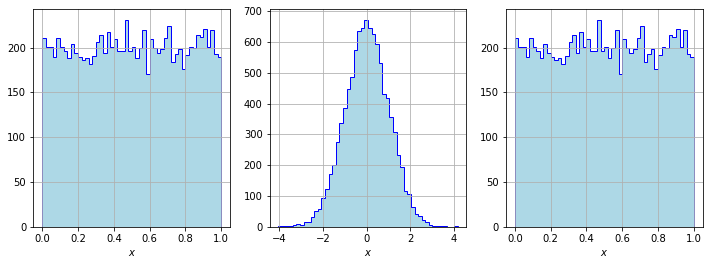
\includegraphics[width=1.\textwidth]{figures/lesson6_11_0.png}
	\caption{Example of transformation, it starts with a uniform distribution, goes into a Gaussian and back to the initial uniform.}
	\label{fig:a:_to_b_to_a}
\end{figure}

\section{Copula}\label{copula}

In probability theory a \emph{copula} \(C(U_1, U_2, \ldots, U_n, \rho)\)
is a multivariate (multidimensional) cumulative distribution function
for which the marginal probability distributions (i.e. the probability
distribution of each dimension) are uniform on the
interval \([0, 1]\) (\(U_i \approx\)uniform(0,1)).
\(\rho\) represent the correlation between each variable.

Copulas are used to describe the dependencies between random variables and
have been widely used in quantitative finance to model risk. Copulas are popular since
they allow to easily model and estimate the distribution of random
vectors by representing marginals and their correlation separately.

Despite the obscure and daunting definition given above the concept of copula is
quite simple so let's try to clarify it a bit with a practical example.

\subsection{Example Problem Case}\label{example-problem-case}

Imagine to measure two variables that are 
correlated. For example, we look at various rivers and for every river
we look at the maximum water level of that river over a certain
time-period. In addition, we also count how many months each river
caused floods.

For the probability distribution of the maximum level of the river we
know that maximums are Gumbel distributed, while the number of floods
can be modeled according to a
\href{https://en.wikipedia.org/wiki/Beta_distribution}{\emph{Beta}}
distribution.

Clearly it is pretty reasonable to assume that the maximum level and the
number of floods is going to be correlated, however we don't know how
we could model that correlated probability distribution.
Above we only
specified the distributions for individual variables, irrespective of
the other one (i.e. the marginals), in reality we are dealing with a
\emph{joint distribution} of both of these together.

And here is where copulas come to our rescue.

Copulas essentially allow to decompose a joint probability distribution
into their marginals (which by definition have no correlation) and a
function which \textbf{couples} (hence the name) them together and thus allows us
to specify the correlation separately. The copula is just that coupling
function.

\subsection{Adding Correlation with Gaussian Copulas}\label{adding-correlation-with-gaussian-copulas}

How does this help us with our problem of creating a custom joint
probability distribution for maximum water level and floods ?

We are actually almost done already, we saw before how to convert
anything uniformly distributed to an arbitrary probability distribution.
So that means we just need to generate uniformly distributed data with the
correlation we want and then transform the marginals into the desired
distributions (Gumbel and Beta in our example).

How do we do that ?

\begin{itemize}
\tightlist
\item
  simulate a sample from a multivariate distribution with the specific correlation structure;
\item
  transform so that the marginals are uniform;
\item
  finally transform the uniform marginals to whatever we like.
\end{itemize}

In this example we sample from a multivariate (2D) normal with a 0.5 correlation, 
see Fig.~ \ref{fig:multivariate_with_correlation}, although this is not mandatory since
we could model correlations with different distribution either.

\begin{tcolorbox}[breakable, size=fbox, boxrule=1pt, pad at break*=1mm,colback=cellbackground, colframe=cellborder]
\begin{Verbatim}[commandchars=\\\{\}]
\PY{n}{mvnorm} \PY{o}{=} \PY{n}{stats}\PY{o}{.}\PY{n}{multivariate\PYZus{}normal}\PY{p}{(}\PY{n}{mean}\PY{o}{=}\PY{p}{[}\PY{l+m+mi}{0}\PY{p}{,} \PY{l+m+mi}{0}\PY{p}{]} \PY{p}{,} \PY{n}{cov}\PY{o}{=}\PY{p}{[}\PY{p}{[}\PY{l+m+mi}{1}\PY{p}{,} \PY{l+m+mf}{0.5}\PY{p}{]}\PY{p}{,}
                                                      \PY{p}{[}\PY{l+m+mf}{0.5}\PY{p}{,} \PY{l+m+mi}{1}\PY{p}{]}\PY{p}{]}\PY{p}{)}
\PY{n}{x} \PY{o}{=} \PY{n}{mvnorm}\PY{o}{.}\PY{n}{rvs}\PY{p}{(}\PY{l+m+mi}{100000}\PY{p}{)}
\end{Verbatim}
\end{tcolorbox}

\begin{figure}[htb]
  \centering
  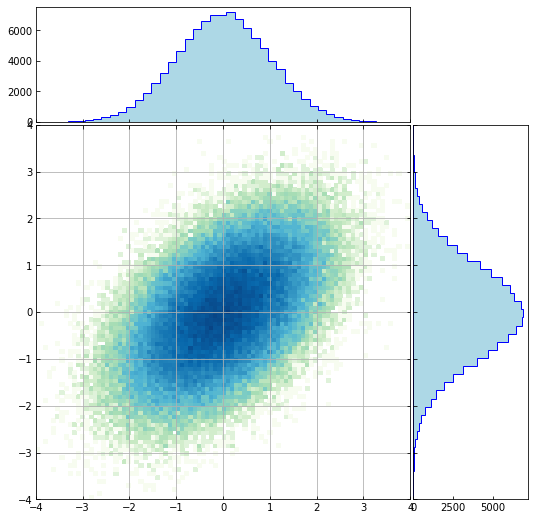
\includegraphics[width=0.5\textwidth]{figures/lesson6_14_0.png}
  \caption{2D multivariate normal distribution with a correlation factor of 0.5.}
  \label{fig:multivariate_with_correlation}
\end{figure}
    
Now use what we have just learned to make the marginals uniform using
the \(\tt{cdf}\) function of the normal distribution:

\begin{tcolorbox}[breakable, size=fbox, boxrule=1pt, pad at break*=1mm,colback=cellbackground, colframe=cellborder]
\begin{Verbatim}[commandchars=\\\{\}]
\PY{n}{norm} \PY{o}{=} \PY{n}{stats}\PY{o}{.}\PY{n}{norm}\PY{p}{(}\PY{p}{)}
\PY{n}{x\PYZus{}unif} \PY{o}{=} \PY{n}{norm}\PY{o}{.}\PY{n}{cdf}\PY{p}{(}\PY{n}{x}\PY{p}{)}
\end{Verbatim}
\end{tcolorbox}

The plots shown in Fig.~\ref{fig:copula} are usually how copulas are visualized.

\begin{figure}[p]
\centering
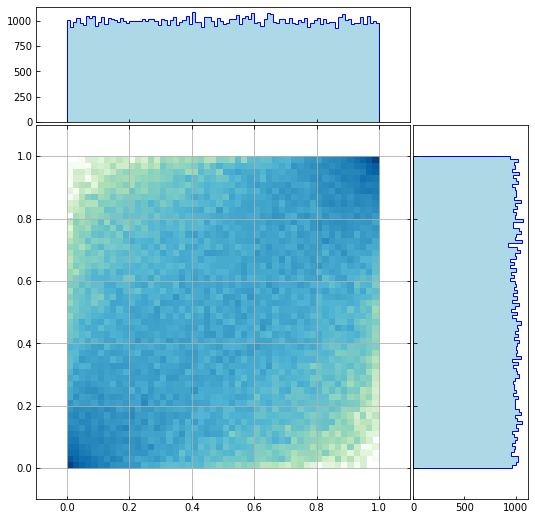
\includegraphics[width=0.45\textwidth]{figures/lesson6_16_0.png}
\quad
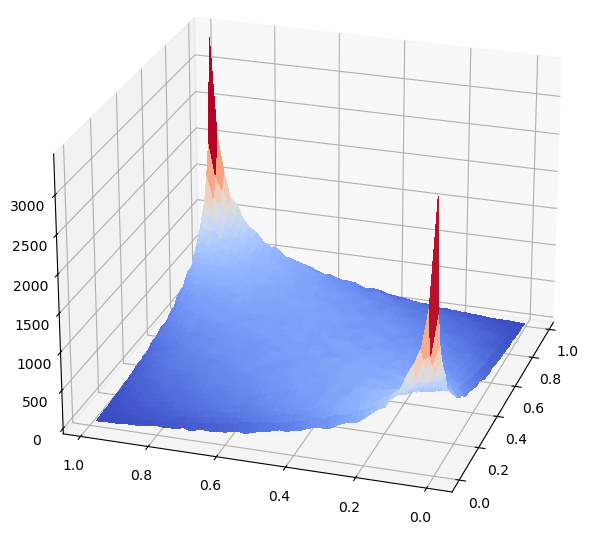
\includegraphics[width=0.5\textwidth]{figures/copula_3d.png}
\caption{Graphical representations of the copula, 2D on the left, 3D on the right.}
\label{fig:copula}
\end{figure}

Finally we can just transform the obtained marginals again from uniform to what we want
(i.e. Gumbel and Beta in our river example):

\begin{tcolorbox}[breakable, size=fbox, boxrule=1pt, pad at break*=1mm,colback=cellbackground, colframe=cellborder]
\begin{Verbatim}[commandchars=\\\{\}]
\PY{n}{m1} \PY{o}{=} \PY{n}{stats}\PY{o}{.}\PY{n}{gumbel\PYZus{}l}\PY{p}{(}\PY{p}{)}
\PY{n}{m2} \PY{o}{=} \PY{n}{stats}\PY{o}{.}\PY{n}{beta}\PY{p}{(}\PY{n}{a}\PY{o}{=}\PY{l+m+mi}{10}\PY{p}{,} \PY{n}{b}\PY{o}{=}\PY{l+m+mi}{3}\PY{p}{)}


\end{Verbatim}
\end{tcolorbox}

Left plot of Figure~\ref{fig:gumbel_beta_with_corr} shows the two marginals and the joint distribution.
    
To see that it is actually working as expected we should now compare the joint
distributions with and without correlation. Compare the two plots in Figure~\ref{fig:gumbel_beta_with_corr} to spot the difference.

\begin{tcolorbox}[breakable, size=fbox, boxrule=1pt, pad at break*=1mm,colback=cellbackground, colframe=cellborder]
\begin{Verbatim}[commandchars=\\\{\}]
\PY{c+c1}{\PYZsh{} sample from Gumbel}
\PY{n}{x1} \PY{o}{=} \PY{n}{m1}\PY{o}{.}\PY{n}{rvs}\PY{p}{(}\PY{l+m+mi}{10000}\PY{p}{)}
\PY{c+c1}{\PYZsh{} sample from Beta}
\PY{n}{x2} \PY{o}{=} \PY{n}{m2}\PY{o}{.}\PY{n}{rvs}\PY{p}{(}\PY{l+m+mi}{10000}\PY{p}{)}
\end{Verbatim}
\end{tcolorbox}

\begin{figure}[p]
  \centering
  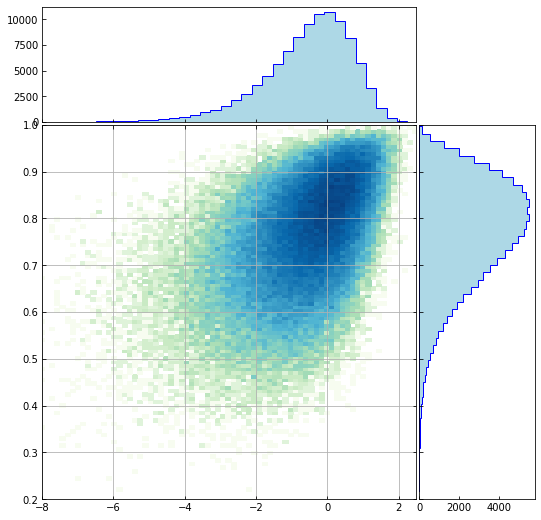
\includegraphics[width=0.45\textwidth]{figures/lesson6_18_0.png}
  \quad
  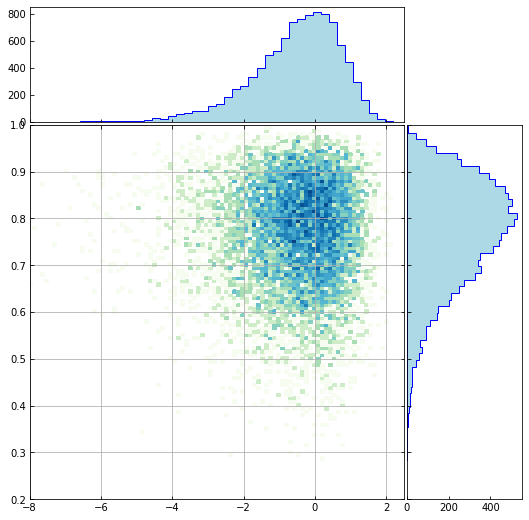
\includegraphics[width=0.45\textwidth]{figures/lesson6_20_0.png}
  \caption{Marginalized Gumbel and Beta distributions and their joint with (left) and without (right) correlation.}
  \label{fig:gumbel_beta_with_corr}
\end{figure}
    
Using the uniform distribution as a common base for our transformations
we can easily introduce correlations and flexibly construct complex
probability distributions. 

As a final note, the \emph{Sklar's theorem} states that any multivariate joint distribution
can be written in terms of uni-variate marginal distribution functions
and a copula which describes the dependence structure between the
variables.

Everything discussed in this Section can be easily generalized to higher dimensions.

%\subsection{Other Copulas}
%In the previous Section we have seen an application of a Gaussian copula but exists many other different 
%kind of copulas. Two typical examples are the t-copula and the Clayton copula.

%\subsubsection{t-copula}

%\subsubsection{Clayton copula}

\subsection{Generate Correlated Distributions}\label{generate-correlated-distributions}

If we need to generate numbers from correlated distribution we can
follow similar steps to those described before:

\begin{itemize}
\tightlist
\item
  generate a random vector \(\mathbf{x}=(x_1, x_2,\ldots)\) from the
  original multivariate distribution;
\item
  determine the single \(U_i(x_i)\) by applying \(\tt{cdf}\) to each
  \(x_i\);
\item
  transform again each \(U_i(x_i)\) to the desired marginal
  distributions using \(\tt{ppf}\);
\item
  each component of the vector \(\mathbf{x}\) is now converted to a set
  of random numbers drawn from the desired distributions, with the
  appropriate correlation.
\end{itemize}

A practical application concerns the probability of default. 
Imagine three companies ($A$, $B$ and $C$) which have a
cumulative probability of defaulting within the next two years of 10\%.
Let's try to compute the probabilities to have the three of them all
defaulting within the next two years in two cases: independent default probabilities and perfectly correlated probabilities.

In the first case (independent probabilities), the
odds to get three defaults within two years will be the product
of the single probabilities, hence:

\[\mathbb{P}_{\mathrm{uncorr}} = 10\% \cdot 10\% \cdot 10\% = 0.1 \%\]

We can verify this in \(\tt{python}\) by applying the method outlined above: first generate a random sample from an uncorrelated multivariate normal distribution, then transform each sampled vector into uniform distribution with the \(\tt{norm.cdf}\) function (i.e. we
convert the samples into cumulative probabilities) and then count how many times the
three of them are lower than 10\% to check whether a default occurred in next two year.

\begin{tcolorbox}[breakable, size=fbox, boxrule=1pt, pad at break*=1mm,colback=cellbackground, colframe=cellborder]
\begin{Verbatim}[commandchars=\\\{\}]
\PY{k+kn}{from} \PY{n+nn}{scipy}\PY{n+nn}{.}\PY{n+nn}{stats} \PY{k}{import} \PY{n}{multivariate\PYZus{}normal}\PY{p}{,} \PY{n}{uniform}\PY{p}{,} \PY{n}{norm}
\PY{k+kn}{import} \PY{n+nn}{numpy}
	
\PY{n}{numpy}\PY{o}{.}\PY{n}{random}\PY{o}{.}\PY{n}{seed}\PY{p}{(}\PY{l+m+mi}{10}\PY{p}{)}
\PY{n}{trials} \PY{o}{=}\PY{l+m+mi}{10000}
\PY{n}{mvnorm\PYZus{}no\PYZus{}corr} \PY{o}{=} \PY{n}{multivariate\PYZus{}normal}\PY{p}{(}\PY{n}{mean}\PY{o}{=}\PY{p}{[}\PY{l+m+mi}{0}\PY{p}{,} \PY{l+m+mi}{0}\PY{p}{,} \PY{l+m+mi}{0}\PY{p}{]}\PY{p}{,} \PY{n}{cov}\PY{o}{=}\PY{p}{[}\PY{p}{[}\PY{l+m+mi}{1}\PY{p}{,} \PY{l+m+mi}{0}\PY{p}{,} \PY{l+m+mi}{0}\PY{p}{]}\PY{p}{,}
                                                          \PY{p}{[}\PY{l+m+mi}{0}\PY{p}{,} \PY{l+m+mi}{1}\PY{p}{,} \PY{l+m+mi}{0}\PY{p}{]}\PY{p}{,}
                                                          \PY{p}{[}\PY{l+m+mi}{0}\PY{p}{,} \PY{l+m+mi}{0}\PY{p}{,} \PY{l+m+mi}{1}\PY{p}{]}\PY{p}{]}\PY{p}{)}
\PY{n}{defaults} \PY{o}{=} \PY{l+m+mi}{0}
\PY{n}{x} \PY{o}{=} \PY{n}{mvnorm\PYZus{}no\PYZus{}corr}\PY{o}{.}\PY{n}{rvs}\PY{p}{(}\PY{n}{trials}\PY{p}{)}
\PY{n}{x\PYZus{}trans} \PY{o}{=} \PY{n}{norm}\PY{o}{.}\PY{n}{cdf}\PY{p}{(}\PY{n}{x}\PY{p}{)}
\PY{k}{for} \PY{n}{i} \PY{o+ow}{in} \PY{n+nb}{range}\PY{p}{(}\PY{n+nb}{len}\PY{p}{(}\PY{n}{x\PYZus{}trans}\PY{p}{)}\PY{p}{)}\PY{p}{:}
    \PY{k}{if} \PY{n}{x\PYZus{}trans}\PY{p}{[}\PY{n}{i}\PY{p}{]}\PY{p}{[}\PY{l+m+mi}{0}\PY{p}{]} \PY{o}{\PYZlt{}} \PY{l+m+mf}{0.1} \PY{o+ow}{and} \PY{n}{x\PYZus{}trans}\PY{p}{[}\PY{n}{i}\PY{p}{]}\PY{p}{[}\PY{l+m+mi}{1}\PY{p}{]} \PY{o}{\PYZlt{}} \PY{l+m+mf}{0.1} \PY{o+ow}{and} \PY{n}{x\PYZus{}trans}\PY{p}{[}\PY{n}{i}\PY{p}{]}\PY{p}{[}\PY{l+m+mi}{2}\PY{p}{]} \PY{o}{\PYZlt{}} \PY{l+m+mf}{0.1}\PY{p}{:}
	\PY{n}{defaults} \PY{o}{+}\PY{o}{=} \PY{l+m+mi}{1}
	
\PY{n+nb}{print} \PY{p}{(}\PY{l+s+s2}{\PYZdq{}}\PY{l+s+s2}{Defaults w/o correlation: }\PY{l+s+si}{\PYZob{}:.2f\PYZcb{}}\PY{l+s+s2}{\PYZpc{}}\PY{l+s+s2}{\PYZdq{}}\PY{o}{.}\PY{n}{format}\PY{p}{(}\PY{n}{defaults}\PY{o}{/}\PY{n}{trials}\PY{o}{*}\PY{l+m+mi}{100}\PY{p}{)}\PY{p}{)}

Defaults w/o correlation: 0.10\%
\end{Verbatim}
\end{tcolorbox}
The result is 0.1\% as expected.

If we repeat the same Monte Carlo experiment with perfectly correlated
default probabilities we have

\begin{tcolorbox}[breakable, size=fbox, boxrule=1pt, pad at break*=1mm,colback=cellbackground, colframe=cellborder]
\begin{Verbatim}[commandchars=\\\{\}]
\PY{n}{mvnorm\PYZus{}corr} \PY{o}{=} \PY{n}{multivariate\PYZus{}normal}\PY{p}{(}\PY{n}{mean}\PY{o}{=}\PY{p}{[}\PY{l+m+mi}{0}\PY{p}{,}\PY{l+m+mi}{0}\PY{p}{,}\PY{l+m+mi}{0}\PY{p}{]}\PY{p}{,} \PY{n}{cov}\PY{o}{=}\PY{p}{[}\PY{p}{[}\PY{l+m+mi}{1}\PY{p}{,} \PY{l+m+mf}{0.999999}\PY{p}{,} \PY{l+m+mf}{0.999999}\PY{p}{]}\PY{p}{,}
                                                     \PY{p}{[}\PY{l+m+mf}{0.999999}\PY{p}{,} \PY{l+m+mi}{1}\PY{p}{,} \PY{l+m+mf}{0.999999}\PY{p}{]}\PY{p}{,}
                                                     \PY{p}{[}\PY{l+m+mf}{0.999999}\PY{p}{,} \PY{l+m+mf}{0.999999}\PY{p}{,} \PY{l+m+mi}{1}\PY{p}{]}\PY{p}{]}\PY{p}{)}
\PY{n}{defaults} \PY{o}{=} \PY{l+m+mi}{0}
\PY{n}{x} \PY{o}{=} \PY{n}{mvnorm\PYZus{}corr}\PY{o}{.}\PY{n}{rvs}\PY{p}{(}\PY{n}{trials}\PY{p}{)}
\PY{n}{x\PYZus{}trans} \PY{o}{=} \PY{n}{norm}\PY{o}{.}\PY{n}{cdf}\PY{p}{(}\PY{n}{x}\PY{p}{)}
\PY{k}{for} \PY{n}{i} \PY{o+ow}{in} \PY{n+nb}{range}\PY{p}{(}\PY{n+nb}{len}\PY{p}{(}\PY{n}{x\PYZus{}trans}\PY{p}{)}\PY{p}{)}\PY{p}{:}
    \PY{k}{if} \PY{n}{x\PYZus{}trans}\PY{p}{[}\PY{n}{i}\PY{p}{]}\PY{p}{[}\PY{l+m+mi}{0}\PY{p}{]} \PY{o}{\PYZlt{}} \PY{l+m+mf}{0.1} \PY{o+ow}{and} \PY{n}{x\PYZus{}trans}\PY{p}{[}\PY{n}{i}\PY{p}{]}\PY{p}{[}\PY{l+m+mi}{1}\PY{p}{]} \PY{o}{\PYZlt{}} \PY{l+m+mf}{0.1} \PY{o+ow}{and} \PY{n}{x\PYZus{}trans}\PY{p}{[}\PY{n}{i}\PY{p}{]}\PY{p}{[}\PY{l+m+mi}{2}\PY{p}{]} \PY{o}{\PYZlt{}} \PY{l+m+mf}{0.1}\PY{p}{:}
        \PY{n}{defaults} \PY{o}{+}\PY{o}{=} \PY{l+m+mi}{1}

\PY{n+nb}{print} \PY{p}{(}\PY{l+s+s2}{\PYZdq{}}\PY{l+s+s2}{Defaults w/ correlation: }\PY{l+s+si}{\PYZob{}:.2f\PYZcb{}}\PY{l+s+s2}{\PYZpc{}}\PY{l+s+s2}{\PYZdq{}}\PY{o}{.}\PY{n}{format}\PY{p}{(}\PY{n}{defaults}\PY{o}{/}\PY{n}{trials}\PY{o}{*}\PY{l+m+mi}{100}\PY{p}{)}\PY{p}{)}

Defaults w/ correlation: 9.89\%
\end{Verbatim}
\end{tcolorbox}
In this case the result is close to 10\%, like we had only one single company. 
Indeed given the perfect correlation between the probabilities either there is no default or three
"simultaneous" defaults with 10\% probability.

\section{Complex Correlation Structures and the Financial
Crisis}\label{complex-correlation-structures-and-the-financial-crisis}

In the example above we have used the multivariate normal distributions which gave
rise to \emph{Gaussian copulas}. However, we could have used other and more complex
copulas as well. For example we might want to assume the correlation is
non-symmetric which is useful in finance when correlations become
very strong during market crashes and returns very negative.

In fact, Gaussian copulas are said to have played a key role in the 2008
financial crisis as tail-correlations were severely underestimated.
Consider a set of mortgages in a CDO (a particular kind of contract that will be introduced in the next Chapter): they are clearly correlated, since if one mortgage fails,
the likelihood that another failing is increased. In the early 2000s,
the banks only knew how to model the marginals of the default rates. Then an
(in)famous paper by Li suggested to use Gaussian copulas to model the
correlations between those marginals. Rating agencies relied on this model so heavily, that severely underestimated the risk and gave false ratings\ldots

If you are interested in the argument read
\href{http://samueldwatts.com/wp-content/uploads/2016/08/Watts-Gaussian-Copula_Financial_Crisis.pdf}{this paper}
for an excellent description of Gaussian copulas and the Financial
Crisis, which argues that different copula choices would not have made a
difference but instead the assumed correlation was way too low.
